%!TEX root = ./intern_report.tex

\newpage
\subsection{Py2WFG: A better way to write Wave Flow Graph}
\subsubsection{Python Vs. WFG}

\begin{figure}[h]
    \centering
    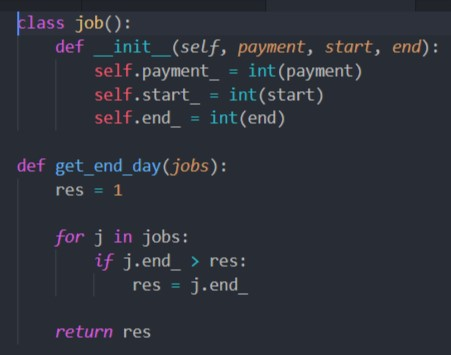
\includegraphics[trim=0cm 0cm 0cm 0cm, clip=true,scale=0.5]{figures/py_eg.jpg}
    \caption{Typical Python code snippet\label{Fig:pyeg}}\vspace{-4mm}
    \end{figure}

\paragraph{}
The Figure~\ref{Fig:pyeg} shows a typical python code example and Figure~\ref{Fig:wfgstruct} shows a WFG snippet. These two languages were built for two entirely different purposes but the highly adaptable nature of python makes a valid point whether if it can replace the functionality of WFG. But both languages have their pros and cons.

\subsubsection*{Python}
\paragraph{}
Python is a general purpose scripting language which focuses on user friendliness. It supports object oriented programming and is also backed up by a huge number of highly optimized libraries for various purposes. But when compared with languages such as C++ and Java, Python is heavy on the memory and slow for large volume computing. It is also not optimized for the particular purpose of programming the Wave DPU.

\subsubsection*{WFG}
\paragraph{}
WFG was created with one purpose and one purpose only in mind, Programming the Wave DPU. Thus it has primary operators that can precisely match the deep capabilities of the DPU hardware. It can be very efficient too when properly programmed. The downside to this language is that it is very strongly typed and is a user friendliness nightmare. Repetitive operators need to be manually entered by the user and the language has no capability of any kind of looping of the language itself.

\subsubsection{Python to WFG translator(Py2WFG)}
\paragraph{}
A solution was created by putting the best of both worlds together. The idea is to create a python 'sleeve' to cover up the WFG interface and present the user with a way to interact with python and get WFG level results. The user will now write up the script and when he runs it, it will output a fully optimized WFG script. 

\begin{figure}[h]
    \centering
    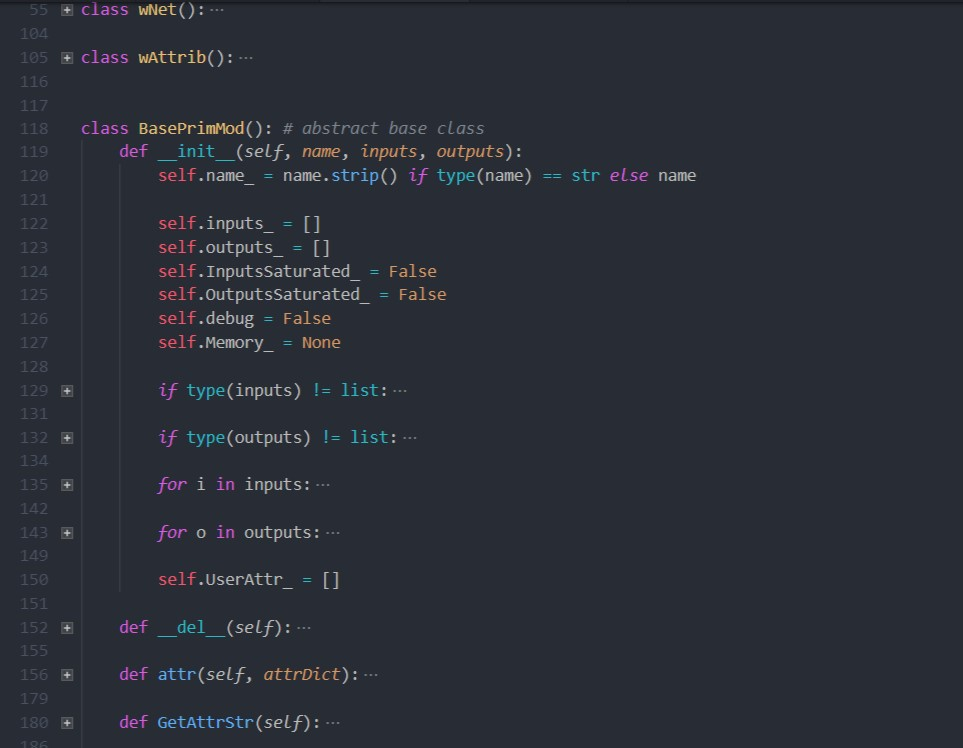
\includegraphics[trim=0cm 0cm 0cm 0cm, clip=true,scale=0.5]{figures/py2wfg_src.jpg}
    \caption{Part of the Py2WFG source code\label{Fig:py2src}}\vspace{-4mm}
    \end{figure}

\subsubsection*{Code Translation}
\paragraph{}
The basic idea for this library is derived from Tensorflow~\cite{tflow}, which is a python library that allows easy neural net design using a python library. The user will still need a sufficient knowledge on WFG syntax to use the library. But it will eliminate the hassles of writing a slightly-above-assembly language scripts by hand. The script that user needs to write is similar to the one showed in Figure~\ref{Fig:py2eg}. The library needs to be imported in to the script, Then Modules can be created from the wMod class in the library. These module 'husks' are then filled with dataflow operations as needed. When complete, issuing the makeWFG command will write a full WFG script that can be later integrated into the existing wave design flow.

\begin{figure}[h]
    \centering
    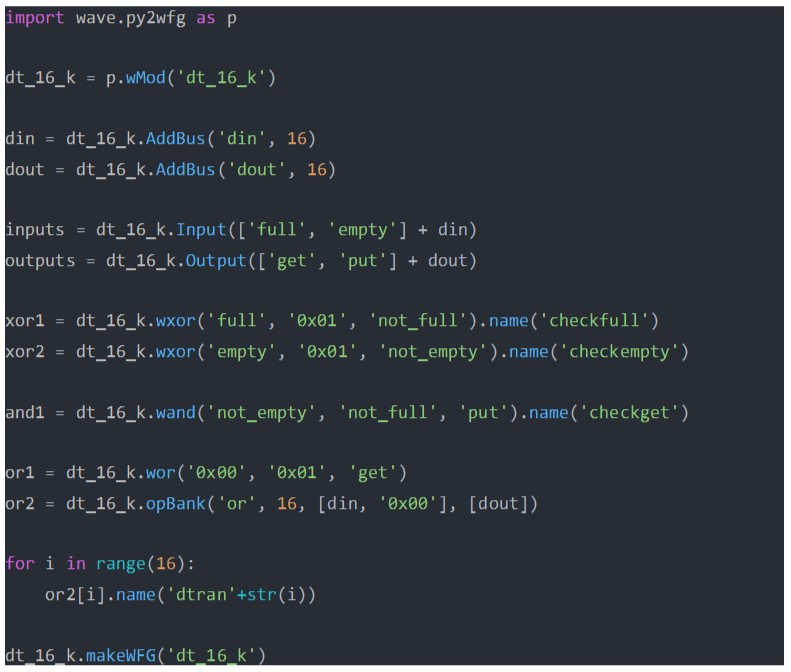
\includegraphics[trim=0cm 0cm 0cm 0cm, clip=true,scale=0.5]{figures/py2wfg_eg.jpg}
    \caption{Example Py2WFG script\label{Fig:py2eg}}\vspace{-4mm}
    \end{figure}

\paragraph{}
Running the example script shown in Figure~\ref{Fig:py2eg} will output a WFG file that contains the operations represented in the script, which is shown in Figure~\ref{Fig:wfgout}

\begin{figure}[h]
    \centering
    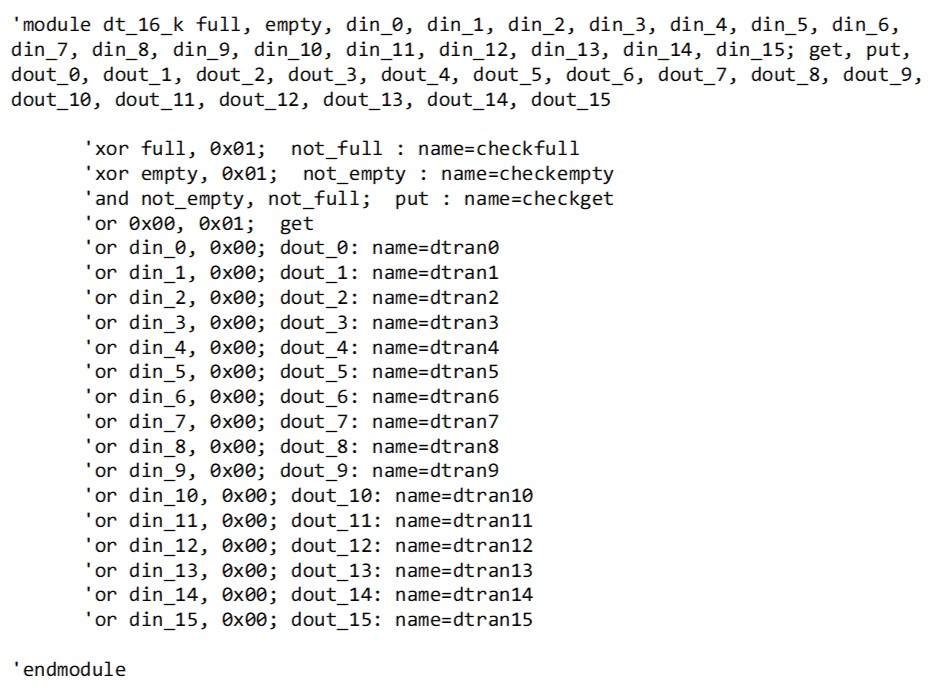
\includegraphics[trim=0cm 0cm 0cm 0cm, clip=true,scale=0.5]{figures/wfg_out.jpg}
    \caption{Output of the Py2WFG code from Figure~\ref{Fig:py2eg}\label{Fig:wfgout}}\vspace{-4mm}
    \end{figure}

\paragraph{}
This output WFG script unlike the handwritten scripts, is properly formatted and can be reconfigured easily through the python script again. This ease of use further improved with the introduction of the Simulator.

\subsubsection{Python to WFG Simulator}
\label{sec:py2wfgsim}

